%%%%%%%%%%%%%%%%%%%%%%%%%%%%%%%%%%%%%%%%%
% Jacobs Landscape Poster
% LaTeX Template
% Version 1.1 (14/06/14)
%
% Created by:
% Computational Physics and Biophysics Group, Jacobs University
% https://teamwork.jacobs-university.de:8443/confluence/display/CoPandBiG/LaTeX+Poster
% 
% Further modified by:
% Nathaniel Johnston (nathaniel@njohnston.ca)
%
% This template has been downloaded from:
% http://www.LaTeXTemplates.com
%
% License:
% CC BY-NC-SA 3.0 (http://creativecommons.org/licenses/by-nc-sa/3.0/)
%
%%%%%%%%%%%%%%%%%%%%%%%%%%%%%%%%%%%%%%%%%


\documentclass[final]{beamer}
\usepackage[scale=1.24]{beamerposter}
\usetheme{confposter}

%-----------------------------------------------------------
% Define the column widths and overall poster size
% To set effective sepwid, onecolwid and twocolwid values, first choose how many columns you want and how much separation you want between columns
% In this template, the separation width chosen is 0.024 of the paper width and a 4-column layout
% onecolwid should therefore be (1-(# of columns+1)*sepwid)/# of columns e.g. (1-(4+1)*0.024)/4 = 0.22
% Set twocolwid to be (2*onecolwid)+sepwid = 0.464
% Set threecolwid to be (3*onecolwid)+2*sepwid = 0.708

\newlength{\sepwid}
\newlength{\onecolwid}
\newlength{\twocolwid}
\newlength{\threecolwid}
\setlength{\paperwidth}{48in} % A0 width: 46.8in
\setlength{\paperheight}{36in} % A0 height: 33.1in
\setlength{\sepwid}{0.024\paperwidth} % Separation width (white space) between columns
\setlength{\onecolwid}{0.22\paperwidth} % Width of one column
\setlength{\twocolwid}{0.464\paperwidth} % Width of two columns
\setlength{\threecolwid}{0.708\paperwidth} % Width of three columns
\setlength{\topmargin}{-0.5in} % Reduce the top margin size
%-----------------------------------------------------------

\usepackage{graphicx}
\usepackage{booktabs}
\title{Stimulus Identification from fMRI scans}

\author{Charles Zheng and Yuval Benjamini} % Author(s)

\institute{Stanford University} % Institution(s)

%----------------------------------------------------------------------------------------

\begin{document}

\addtobeamertemplate{block end}{}{\vspace*{2ex}} % White space under blocks
\addtobeamertemplate{block alerted end}{}{\vspace*{2ex}} % White space under highlighted (alert) blocks

\setlength{\belowcaptionskip}{2ex} % White space under figures
\setlength\belowdisplayshortskip{2ex} % White space under equations

\begin{frame}[t] % The whole poster is enclosed in one beamer frame

\begin{columns}[t] % The whole poster consists of three major columns, the second of which is split into two columns twice - the [t] option aligns each column's content to the top

\begin{column}{\sepwid}\end{column} % Empty spacer column

\begin{column}{\onecolwid} % The first column

%----------------------------------------------------------------------------------------
%	INTRODUCTION
%----------------------------------------------------------------------------------------
\begin{block}{Setting}
\begin{itemize}
\item Sequence of stimuli (pictures) shown at time $t = 1,\hdots, T$
\item Record subject's multivariate response $Y_t \in \mathbb{R}^p$
\item Stimuli represented as \emph{feature vector} $X_t \in \mathbb{R}^q$
\item Linear model:
\[
Y_{T \times p} = X_{T \times q} B_{q \times p} + E_{T \times p}
\]
\item E.g. Kay (2008)
\end{itemize}

\begin{center}
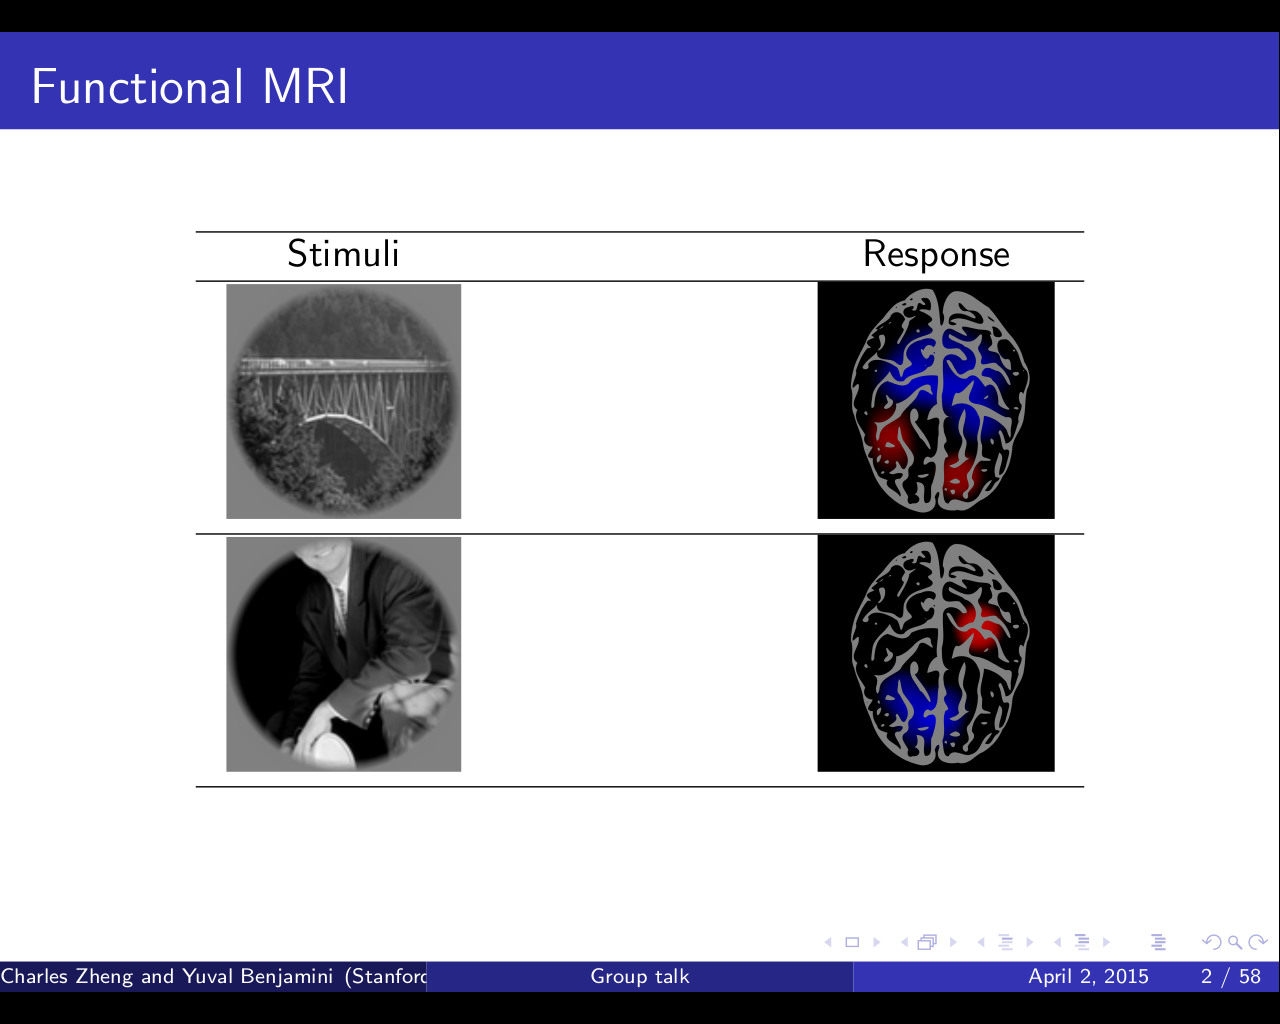
\includegraphics[scale = 0.5, trim=3in 3in 3in 3in, clip]{screen1.png}
\end{center}
\end{block}

\begin{block}{Identification}
\begin{itemize}
\item Introduced in Kay (2008)
\item Supervised learning task, validates the power of the linear model $Y = XB + E$
\item Let $S$ be a set of \emph{new} stimuli (not in the training set) with features
\[
\{x_1^{te}, \hdots, x_\ell^{te}\}
\]
\item Scientist picks a stimulus $i^*$ from $S$ and measures the subject's reponse $y^*$
\item Can the statistician \emph{identify} the stimulus from $y^*$?
\end{itemize}
\begin{center}
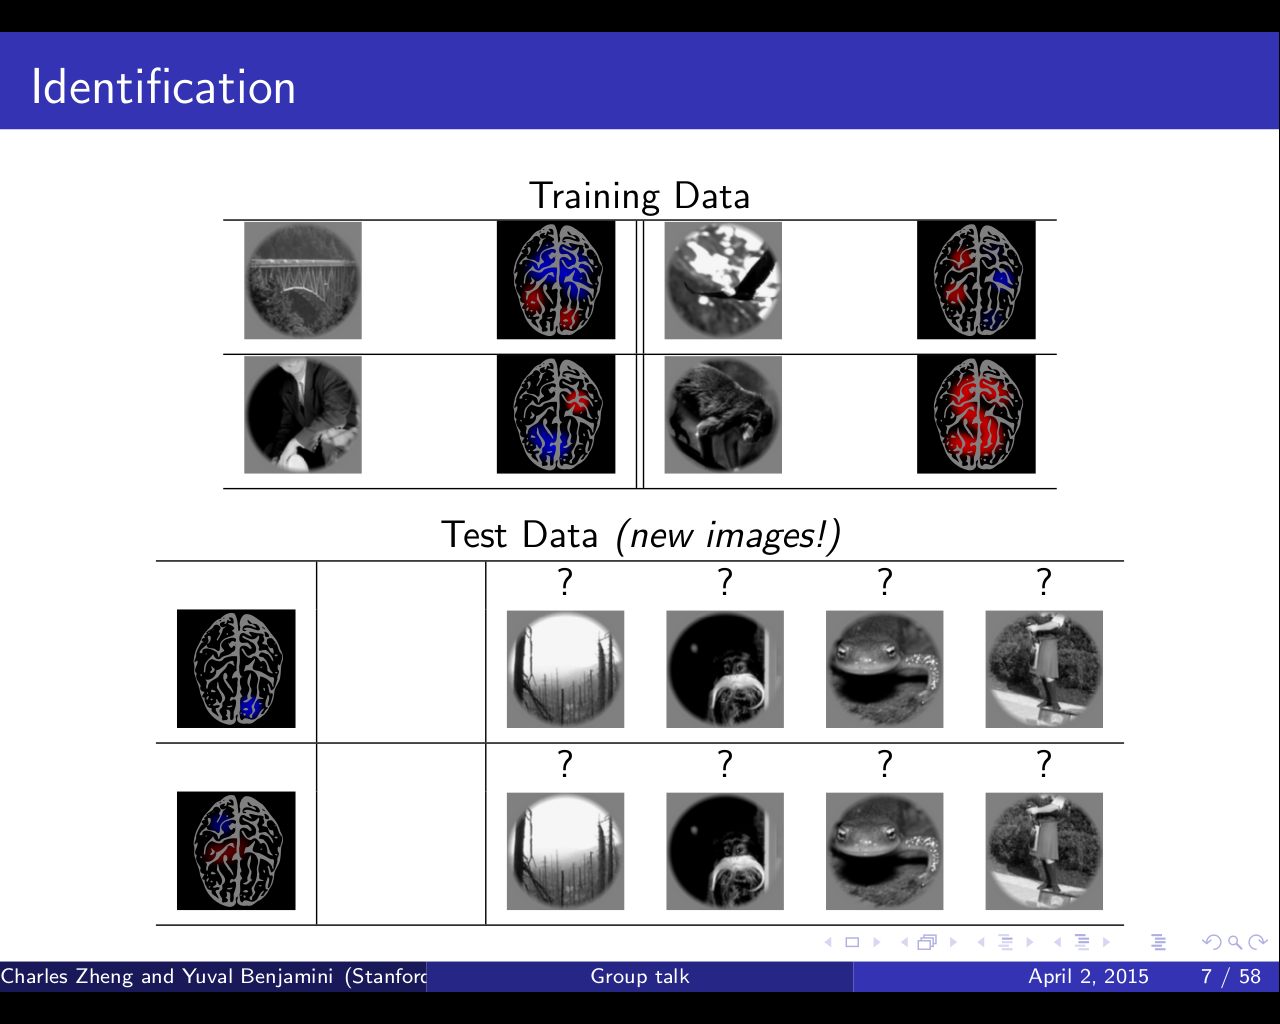
\includegraphics[scale = 0.5, trim=1in 1.5in 1in 2in, clip]{screen4.png}
\end{center}
\end{block}

\end{column} % End of the first column

\begin{column}{\sepwid}\end{column} % Empty spacer column



\begin{column}{\onecolwid}

%----------------------------------------------------------------------------------------
%	MATERIALS
%----------------------------------------------------------------------------------------

\begin{block}{Objectives}
\begin{itemize}
\item Develop new methodology for optimal identification
\end{itemize}

\emph{Key theoretical problems:}
\begin{itemize}
\item Optimal identification given parameter estimates
\item Estimation of model (e.g. linear model $Y = XB$)
\item Estimation of noise $\Sigma_E = \text{Cov}(E)$
\end{itemize}

\emph{Optimality criteria:}
\begin{itemize}
\item Bayes (average case) under parametric models
\item Minimax regret under nonparametric models
\end{itemize}

We consider two methods: \emph{maximum likelihood} and \emph{empirical
  Bayes}, and compare to \emph{Bayes risk}.
\end{block}



\begin{block}{Maximum Likelihood}

Procedure for identification of $y^*$,
variants used in Kay (2008), Vu (2011)

\begin{itemize}
\item Obtain point estimates of coefficients $B$ and noise covariance $\Sigma_E$
\item E.g. $B$ estimated using elastic net with CV (Zou 2005),
shrinkage estimate for covariance
\[
\hat{\Sigma}_E = \frac{1}{2}\hat{\text{Cov}}(Y - \hat{Y}) + \frac{1}{2}\text{diag}(\hat{\text{Cov}}(Y - \hat{Y}))
\]
where $\hat{\text{Cov}}$ denotes sample covariance
\item Obtain predicted means for test stimuli
\[
\hat{\mu}_i^{te} = (x_i^{te})^T B
\]
\item Identify the stimulus $i^*$ by
\[
i^* = \text{argmin}_{i} (\hat{\mu}_i^{te} - y^*)^T \hat{\Sigma}_E^{-1} (\hat{\mu}_i^{te} - y^*)
\]
\item Results in \emph{linear decision boundaries}
\end{itemize}

\begin{center}
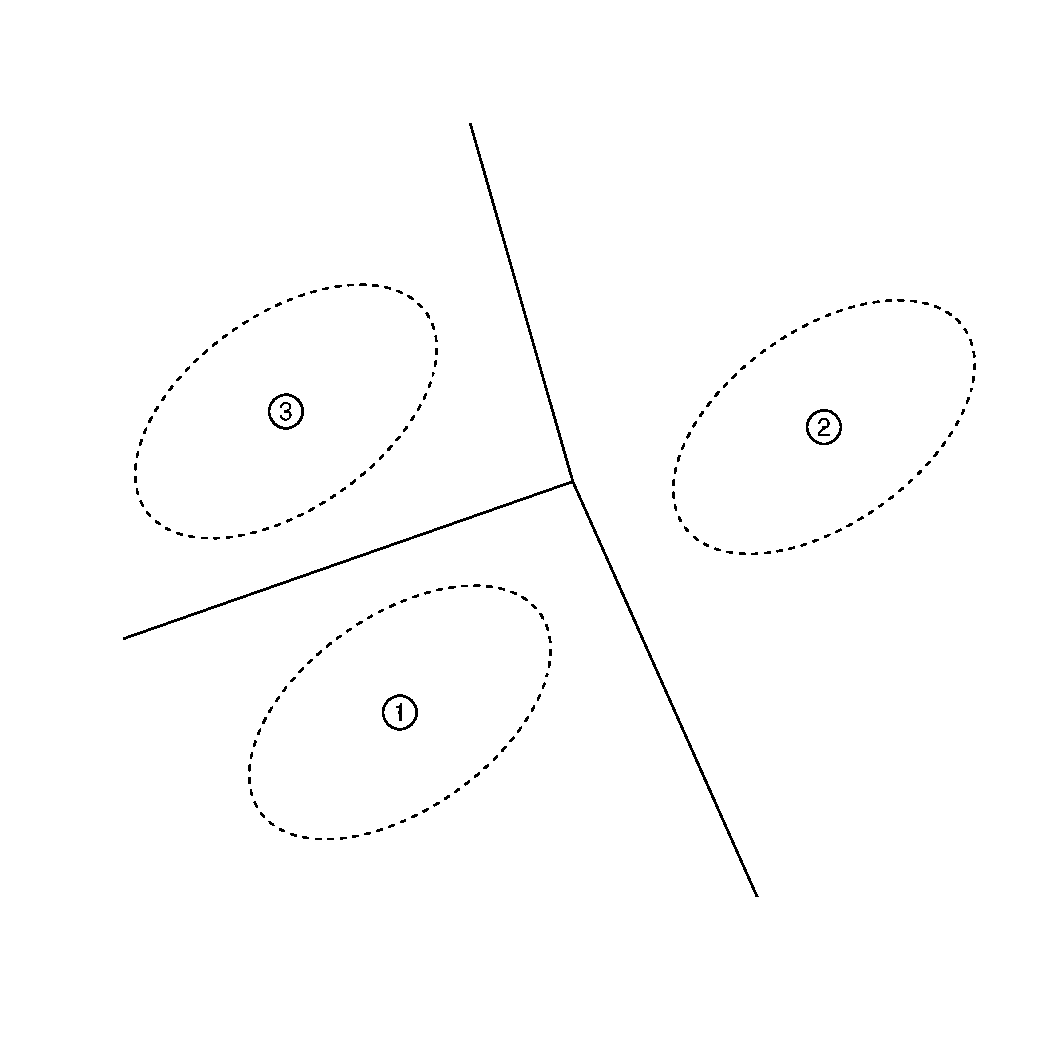
\includegraphics[scale = 1.0]{illus1_A.pdf}
\end{center}

%\emph{Theoretical results}
%\begin{itemize}
%\item Asymptotic consistency to optimal procedure $T \to \infty$ under correct model specification
%\item Inconsistency given model misspecification (nonlinearity)
%\end{itemize}

\end{block}

%----------------------------------------------------------------------------------------

\end{column} % End of column 2.1

\begin{column}{\sepwid}\end{column} % Empty spacer column


\begin{column}{\onecolwid}

%----------------------------------------------------------------------------------------
%	METHODS
%----------------------------------------------------------------------------------------
\begin{alertblock}{What is Empirical Bayes?}
\begin{itemize}
\item General approach for statistical problems (e.g. Efron 2004)
\item Start with a hierarchical Bayes model with hyperparameters
\item \emph{Estimate} hyperparameters from data, e.g. maximizing marginal likelihood
\end{itemize}
\end{alertblock}

\begin{block}{Empirical Bayes}

\emph{Model}

\begin{itemize}
\item Noise $E_t \sim N(0, \Sigma_E)$ iid 
\item Coefficients $B_i \sim N(0, \sigma^2_i I)$ for $i = 1, \hdots, p$
\item $X$ non-random
\end{itemize}

\emph{Estimate hyperparameters}

\begin{itemize}
\item Use \emph{eigenprism} (Janson 2015) to estimate $\theta_i^2 = ||B_i||^2$ for $i =1,\hdots, p$
\item Set $\sigma^2_i = \hat{\theta}_i^2/q$
\item Estimate $\hat{B}$ as posterior mean given estimated $\sigma^2_i$
\item Estimate $\Sigma_E$ using residuals (same as in Maximum Likelihood)
\end{itemize}

\emph{Compute posterior}
\begin{itemize}
\item Closed-form expressions for posteriors of $B$, $\mu_i^{te}$
\item Computational bottleneck: inverting the $pq \times pq$ covariance matrix of $\vec{B}$
\end{itemize}

\emph{Apply Bayes rule}

\begin{itemize}
\item \emph{Uncertainty} in $B$ is reflected as \emph{added noise}
\item Result: posterior $\text{Cov}(y^*|i^*)$ varies, hence \emph{quadratic boundaries}
\end{itemize}

\begin{center}
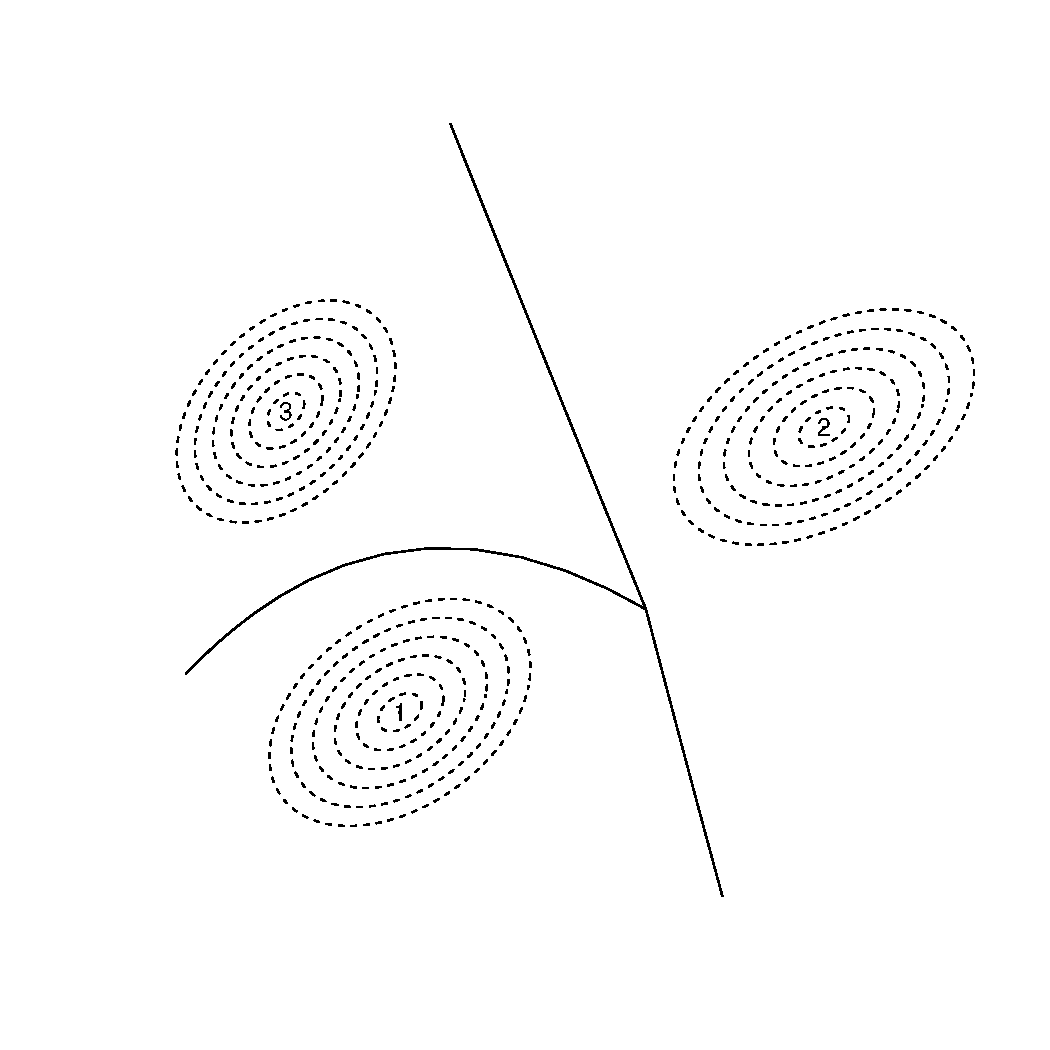
\includegraphics[scale = 1.0]{illus1_B.pdf}
\end{center}

\end{block}


%----------------------------------------------------------------------------------------

\end{column} % End of column 2.2

\begin{column}{\sepwid}\end{column} % Empty spacer column

\begin{column}{\onecolwid} % The third column

%----------------------------------------------------------------------------------------
%	CONCLUSION
%----------------------------------------------------------------------------------------

\begin{block}{Simulation Results}

\end{block}

\begin{block}{Ongoing Work}
\begin{itemize}
\item Estimate noise covariance based on correlation structure of fMRI data (e.g. spatial correlation)
\item Apply methods to data of Kay (2008)
\end{itemize}
\end{block}

%----------------------------------------------------------------------------------------
%	REFERENCES
%----------------------------------------------------------------------------------------

\begin{block}{References}

\nocite{*} % Insert publications even if they are not cited in the poster
\small{\bibliographystyle{unsrt}
\bibliography{sample}\vspace{0.75in}}

\end{block}

%----------------------------------------------------------------------------------------
%	ACKNOWLEDGEMENTS
%----------------------------------------------------------------------------------------

\setbeamercolor{block title}{fg=red,bg=white} % Change the block title color

\begin{block}{Acknowledgements}

\small{\rmfamily{Nam mollis tristique neque eu luctus. Suspendisse rutrum congue nisi sed convallis. Aenean id neque dolor. Pellentesque habitant morbi tristique senectus et netus et malesuada fames ac turpis egestas.}} \\

\end{block}

%----------------------------------------------------------------------------------------
%	CONTACT INFORMATION
%----------------------------------------------------------------------------------------

\setbeamercolor{block alerted title}{fg=black,bg=norange} % Change the alert block title colors
\setbeamercolor{block alerted body}{fg=black,bg=white} % Change the alert block body colors

\begin{alertblock}{Contact Information}

\begin{itemize}
\item Web: \href{http://www.university.edu/smithlab}{http://www.university.edu/smithlab}
\item Email: \href{mailto:john@smith.com}{john@smith.com}
\item Phone: +1 (000) 111 1111
\end{itemize}

\end{alertblock}

\begin{center}
\begin{tabular}{ccc}

\includegraphics[width=0.4\linewidth]{logo.png} & \hfill & 
\includegraphics[width=0.4\linewidth]{logo.png}
\end{tabular}
\end{center}

%----------------------------------------------------------------------------------------

\end{column} % End of the third column

\end{columns} % End of all the columns in the poster

\end{frame} % End of the enclosing frame

\end{document}
